\chapter{Introduction}\label{chap:introduction}
Semantic segmentation is a popular research topic in the field of computer vision, and particularly for autonomous vehicles.
The ability to semantically understand a scene is important for autonomous vehicles and robots to safely navigate an environment.
Generally, most implementations attempt to segment road surfaces but in this thesis, we propose the segmentation of curbs and curb cuts to allow safer sidewalk navigation.

The Europa project has resulted in the Obelix robotic platform, which has already been demoed to successfully perform pedestrian navigation~\cite{europa}\cite{obelix-slam}.
We propose to add to this platform the ability to detect curbs and curb cuts using semantic segmentation.
The Obelix platform is the result of a joint project to build a robotic platform capable of robotic navigation~\cite{europa}. 
In its current state, Obelix is already capable of localization and navigation using a map generated using LIDAR, but it is unable to determine what surface type it is driving on, e.g. asphalt, concrete, carpet, etc.~\cite{jannik}.
To extend its pathfinding ability, a project is currently underway to use the stereo cameras to classify surfaces that Obelix will encounter~\cite{jannik}.
This work specifically aims to add to said project by additionally identifying curbs and curb cuts, providing constraints for the route planner.
This will allow the route planner to identify curbs, which it cannot traverse, and curb cuts, which it can.

\begin{figure}
	\centering
	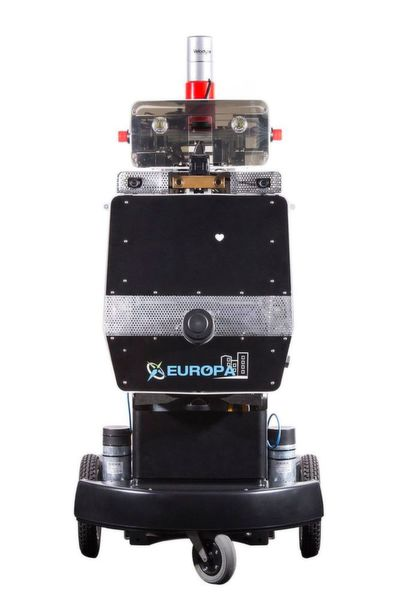
\includegraphics[width=.3\textwidth]{figures/introduction/obelix.jpg}
	\caption{The Obelix Robot platform developed by the Europa project. We plan to extend its path finding capabilities using the work in this thesis.}
\end{figure}

Our goal is thus to implement a computer vision algorithm capable of the semantic segmentation of curbs and curb cuts using a single camera image.
To do so, we implement a convolutional neural network (CNN) based on the paper "Encoder-Decoder with Atrous Separable Convolution for Semantic Image Segmentation" by Chen Liang Chieh et al~\cite{deeplab}.
We additionally include prior knowledge to the training, as it can be assumed that the camera setup and attitude for Obelix will remain relatively constant throughout its lifespan.

This thesis begins by discussing the motivation behind this thesis, followed by a discussion of related works and the background.
The approach is then discussed in detail along with the experiments and results.
Finally, a discussion of potential future research is be presented followed by the conclusion.
